%   % !TEX root = ../../VIII,3_Rahmen-TeX_8-1.tex
%
%
%   Band VIII, 3 N.~??S01.02
%   Signatur/Tex-Datei: LH_35_09_23_003,006
%   RK-Nr. 41208 /2
%   \ref{dcc_02-1}
%   Überschrift: De corporum concursus scheda secunda
%   Modul: Mechanik / Stoß ()
%   Datierung: Januar 1678
%   WZ: LEd-WZ 803003 = RK-WZ 142 (eins)
%   SZ: %\leibdashv %\leibvdash (zwei)
%   Bilddateien (PDF): LH_35_09_23_003,006_d01; LH_35_09_23_003,006_d02; LH_35_09_23_003,006_d03; LH_35_09_23_003,006_d1; LH_35_09_23_003,006_d2; LH_35_09_23_003,006_d3; LH_35_09_23_003,006_d4 (insgesamt: sieben)
%   Verzeichniseinträge: vollständig
%   \textls{} statt \textso{} (Ausnahme: Personenverzeichnis)
%
%
\selectlanguage{ngerman}%
\frenchspacing%
%
\begin{ledgroupsized}[r]{120mm}%
\footnotesize%
\pstart%
\noindent\textbf{Überlieferung:}%
\pend%
\end{ledgroupsized}%
\begin{ledgroupsized}[r]{114mm}%
\footnotesize%
\pstart%
\parindent -6mm
\makebox[6mm][l]{\textit{L}}%
Konzept: LH XXXV 9, 23 Bl.~3,~6.
Ein Bogen 2\textsuperscript{o},
den Träger von N.~\ref{dcc_02-2} %??S01\textsubscript{3} 
umschließend;
ein Wasserzeichen auf Bl.~3.
Vier vollbeschriebene Seiten, die den Text N.~\ref{dcc_01} %??S01\textsubscript{1} 
fortsetzen und vom Text N.~\ref{dcc_03} %??S01\textsubscript{4} 
fortgesetzt werden.
Randbemerkungen zum Teil \textit{post reformationem} verfasst (siehe die editorische Vorbemerkung, S.~\refpassage{dcc_Vorbemerkung_reform-1}{dcc_Vorbemerkung_reform-2}).
\pend%
\end{ledgroupsized}%
%
\begin{ledgroupsized}[r]{114mm}%
\footnotesize%
\pstart%
\parindent -6mm%
\makebox[6mm][l]{\textit{E}}%
\textsc{Fichant}\cite{01056} 1994, S.~80\textendash88
(mit kommentierter französischer Übersetzung, S.~200\textendash207).

\pend%
\end{ledgroupsized}%
%
\selectlanguage{latin}%
\frenchspacing%
%
\count\Bfootins=1200%
\count\Afootins=1200%
\count\Cfootins=1200%
%
\vspace{8mm}%
\normalsize%
\pstart%
\noindent%
%
\lbrack3~r\textsuperscript{o}\rbrack% \ % % % % Blatt 3r
%
\phantom{Januar. 1678}%
\hfill%
De corporum concursu%
\protect\index{Sachverzeichnis}{concursus corporum}
\hfill%
\phantom{\lbrack3~r\textsuperscript{o}\rbrack}%
Januar. 1678
\pend%
%
\pstart%
\noindent%
\centering%
Scheda secunda\protect\index{Sachverzeichnis}{scheda}
\pend%
\vspace{0.5em}%
%
\pstart%
\noindent%
Paulatim a simplicissimis inchoando
ita profecimus in hoc argumento,%
\protect\index{Sachverzeichnis}{argumentum}
ut jam teneamus
quae sint corporum aequalium concurrentium%
\protect\index{Sachverzeichnis}{corpora concurrentia aequalia}
quomodocunque leges;%
\protect\index{Sachverzeichnis}{lex concursus}
sed et quid contingat,
quando corpus majus et celerius%
\protect\index{Sachverzeichnis}{corpus incurrens}%
\protect\index{Sachverzeichnis}{corpus majus in minus}%
\protect\index{Sachverzeichnis}{corpus celerius}
incurrit in minus et tardius%
\protect\index{Sachverzeichnis}{corpus tardius}
(qui erat casus%
\protect\index{Sachverzeichnis}{casus concursuum}
post aequalitatem facillimus);
\edlabel{LH_35_09_23_003r_jhgmg-1}%
nunc definiendum est,
quid fiat
quando corpus minus et celerius
incurrit in majus et tardius%
\protect\index{Sachverzeichnis}{corpus minus in majus}%
\edlabel{LH_35_09_23_003r_jhgmg-2}
(\protect\vphantom)%
nam tardius in celerius incurrere
seu ipsum assequi non potest%
\protect\vphantom().
Hunc autem
%
\edtext{casum ut solvere tentaremus assumseramus}{%
\lemma{casum}\Bfootnote{%
\textit{(1)}~ut solvamus, assumendum est
\textit{(2)}~ut solvere tentaremus assumseramus%
~\textit{L}}}
%
\edlabel{LH_35_09_23_003r_Lemmainversionis-1}%
Lemma,\protect\index{Sachverzeichnis}{lemma inversionis}
quod elegans videtur,
et omnibus primo aspectu rationi consentaneum videbitur.
Si duo corpora post concursum a se invicem recedentia,%
\protect\index{Sachverzeichnis}{corpus recedens}
eadem qua discedunt celeritate%
\protect\index{Sachverzeichnis}{celeritas discessus}
in locum concursus%
\protect\index{Sachverzeichnis}{locus concursus}
redire intelligantur,
tunc post hunc novum concursum%
\protect\index{Sachverzeichnis}{concursus novus}
redibitur in statum
qui erat ante primum concursum.%
\protect\index{Sachverzeichnis}{concursus primus}%
\edlabel{LH_35_09_23_003r_Lemmainversionis-2}
Hoc Lemma praeterquam
%
\edtext{quod experimentis%
\protect\index{Sachverzeichnis}{experimentum}}{%
\lemma{quod}\Bfootnote{\hspace{-0,5mm}%
\textbar~in \textit{streicht Hrsg.}~%
\textbar\ experimentis}}
%
quibusdam jam
%
\edtext{apud alios sumtis}{%
\lemma{apud alios sumtis}\Cfootnote{%
Vgl. etwa E.~\textsc{Mariotte}, \textit{Traité de la percussion}, partie I, prop. 20 (Paris 1673, S.~122; 125\,f.);\cite{00311}
% auch Huygens; 
hierüber \textsc{Fichant} 1994, S.~202.\cite{01056}
Leibniz hatte die Stelle in Paris exzerpiert (vgl. \textit{LSB} VIII,~2 N.~50, S.~433.1\textendash5\cite{01292}) und sich auch später mit ihr befasst:
Vgl. N.~\ref{RK57267-3} in diesem Band, S.~\refpassage{LH_37_05_145r_prop.I.20_Mario-1}{LH_37_05_145r_prop.I.20_Mario-2}.%
}}
%
consonat\lbrack,\rbrack\
etiam attente
%
\edtext{consideranti probabile apparebit\lbrack;\rbrack}{%
\lemma{consideranti}\Bfootnote{%
\textit{(1)}~necessarium apparebat
\textit{(2)}~probabile apparebit,%
~\textit{L}}}
%
nam effectus omnis causam suam reproducere potest.%
\protect\index{Sachverzeichnis}{effectus causam reproducens}
%
\edtext{Et quando facile demonstrari potest}{%
\lemma{Et}\Bfootnote{%
\textit{(1)}~cum facile demonstrari possit
\textit{(2)}~quando facile demonstrari potest%
~\textit{L}}}
%
debere per regressum hunc%
\protect\index{Sachverzeichnis}{regressus}
prodire aliquid valde affine primo statui,%
\protect\index{Sachverzeichnis}{status primus}
tunc nulla poterit ratio reddi%
\protect\index{Sachverzeichnis}{ratio reddenda}
%
\edtext{cur aliud}{%
\lemma{cur}\Bfootnote{\hspace{-0,5mm}%
\textbar~non \textit{gestr.}~%
\textbar\ aliud%
~\textit{L}}}
%
potius,
quam illud ipsum.
Quae ratiocinatio\protect\index{Sachverzeichnis}{ratiocinatio}
apud me vim habet demonstrationis.%
\protect\index{Sachverzeichnis}{vis demonstrationis}
Et
%
\edtext{paulo ante}{%
\lemma{paulo ante}\Cfootnote{%
Siehe N.~\ref{dcc_01}, %??S01\textsubscript{1}, 
S.~\refpassage{LH_35_09_23_001v_celeritatibuspermutatis-1}{LH_35_09_23_001v_celeritatibuspermutatis-2}.}}
%
etiam a me adhibita est,
cum in aequalibus corporibus ostenderem permutationem celeritatis.%
\protect\index{Sachverzeichnis}{permutatio celeritatis}
Sed ut Lemma%
\protect\index{Sachverzeichnis}{lemma inversionis}
%
\edtext{hoc melius intelligatur,
applicabimus}{%
\lemma{hoc}\Bfootnote{%
\textit{(1)}~ejusque applicatio
\textit{(2)}~melius intelligatur, applicabimus%
~\textit{L}}}
%
ipsum ad casum de quo agitur.
\pend%
%
\pstart%
Sit%
\edlabel{LH_35_09_23_003r_BezugFig4_fgkh-1}
%
\edtext{fig.~4 ad}{%
{\lemma{fig.~4}\Bfootnote{%
\textit{(1)}~ex
\textit{(2)}~ad%
~\textit{L}}}%
{\lemma{fig.~4}\Cfootnote{%
Siehe N.~\ref{dcc_01}, %??S01\textsubscript{1}, 
S.~\pageref{LH_35_09_23_001-002_Fig.6}, Diagramm \lbrack\textit{Fig.~6}\rbrack.}}}
%
amussim respondens\protect\index{Sachverzeichnis}{figura}
%
\edtext{figurae~3,}{%
\lemma{figurae~3}\Cfootnote{%
Siehe N.~\ref{dcc_01}, %??S01\textsubscript{1}, 
S.~\pageref{LH_35_09_23_001-002_Fig.5}, Diagramm \lbrack\textit{Fig.~5}\rbrack.}}
%
ita ut tantum \textit{B} minus antea excipiens,%
\protect\index{Sachverzeichnis}{corpus minus excipiens}
fiat nunc incurrens,%
\protect\index{Sachverzeichnis}{corpus minus incurrens}
et \textit{A} majus antea incurrens%
\protect\index{Sachverzeichnis}{corpus majus incurrens}
fiat nunc excipiens.%
\protect\index{Sachverzeichnis}{corpus majus excipiens}
Et loca post concursum%
\protect\index{Sachverzeichnis}{locus post concursum}
intelligantur esse loca ante concursum%
\protect\index{Sachverzeichnis}{locus ante concursum}
et contra.
Hoc modo enim nihil in figura mutandum%
\protect\index{Sachverzeichnis}{figura}
%
\edtext{est,
nisi in literarum%
\protect\index{Sachverzeichnis}{litera}
et corporum punctationibus,%
\protect\index{Sachverzeichnis}{punctuatio}}{%
\lemma{est,}\Bfootnote{%
\textit{(1)}~tantum
\textit{(a)}~pro
\textit{(b)}~in literis
\textit{(2)}~nisi in
\textit{(a)}~literis et
\textit{(b)}~literarum et corporum punctationibus,%
~\textit{L}}}
\pend
%
\pstart%
\noindent%
nempe pro
\!\raisebox{-3,6mm}{$\displaystyle\efrac{\textit{((B))}}{\displaystyle\efrac{\textit{((A))}}{\textit{((C))}}}$}
fit
\raisebox{-3,6mm}{$\displaystyle\efrac{\protect\vphantom{\textit{((}}B\protect\vphantom{\textit{))}}}{\displaystyle\efrac{\protect\vphantom{\textit{((}}A\protect\vphantom{\textit{))}}}{\protect\vphantom{\textit{((}}C\protect\vphantom{\textit{))}}}}$}
et contra,
\pend
\vspace{1,5mm}
%
\pstart%
\noindent%
\raisebox{5,5mm}{et pro}
%
\includegraphics[width=0.042\textwidth]{gesamttex/edit_VIII,3/images/LH_35_09_23_003,006_d0a.pdf}
%
\raisebox{5,5mm}{fit}
%
\includegraphics[width=0.04\textwidth]{gesamttex/edit_VIII,3/images/LH_35_09_23_003,006_d0b.pdf}
%
\raisebox{5,5mm}{et contra,}%
% \rule[0mm]{0mm}{0mm}
\pend
\vspace{-0,6mm}
%
\pstart%
\noindent%
\raisebox{1,5mm}{manent vero \textit{(A), (B), (C)} et}
%
\includegraphics[width=0.080\textwidth]{gesamttex/edit_VIII,3/images/LH_35_09_23_003,006_d0c.pdf}
%
\raisebox{1,8mm}{.}
\pend
%
\pstart
Id est ponamus in fig.~3. corpus
%
\edtext{majus}{%
\lemma{majus}\Bfootnote{%
\textit{erg.~L}}}
%
\textit{A} celeritate \textit{A(A)}%
\protect\index{Sachverzeichnis}{celeritas corporis concurrentis}
incurrisse in corpus
%
\edtext{minus}{%
\lemma{minus}\Bfootnote{%
\textit{erg.~L}}}
%
\textit{B} ipsum praecedens celeritate \textit{B(B)},
locum concursus\protect\index{Sachverzeichnis}{locus concursus} esse 
%
\edtext{\lbrack puncta\rbrack}{\lemma{punctum}\Bfootnote{\textit{L~ändert Hrsg.}}}
%
\textit{(A)},\,\textit{(B)}
%
\edtext{quae pono}{%
\lemma{quae}\Bfootnote{%
\textit{(1)}~ponimus
\textit{(2)}~pono%
~\textit{L}}}
%
coincidere,
quia compendii causa%
\protect\index{Sachverzeichnis}{compendium}
%
\edtext{ut supra dixi}{%
\lemma{ut supra dixi}\Cfootnote{%
N.~\ref{dcc_01}, %??S01\textsubscript{1},
S.~\pageref{LH_35_09_23_002v_MargCoincidunt}, Randbemerkung.
Siehe zudem
S.~\refpassage{LH_35_09_23_002v_PunctaCoincidunt_wdm-1}{LH_35_09_23_002v_PunctaCoincidunt_wdm-2}.}}
%
\edtext{corpora perinde considero
ac si in punctum salvo pondere%
\protect\index{Sachverzeichnis}{pondus corporis concurrentis}
(\protect\vphantom)%
quod appicta magnitudine exprimitur%
\protect\vphantom()
redacta essent.}{%
\lemma{corpora}\Bfootnote{%
\textit{(1)}~in rat
\textit{(2)}~perinde considero \lbrack...\rbrack\ redacta essent.%
~\textit{L}}}
%
Post concursum vero
%
\edtext{ut ostendimus}{%
\lemma{ut ostendimus}\Cfootnote{%
Siehe N.~\ref{dcc_01}, %??S01\textsubscript{1},
S.~\refpassage{LH_35_09_23_002v_utostedimus_hik-1}{LH_35_09_23_002v_utostedimus_hik-2}.}}
%
corpus \textit{B} progredi celeritate \textit{(B)((B))},%
\protect\index{Sachverzeichnis}{celeritas corporis concurrentis}
corpus vero \textit{A} celeritate \textit{(A)((A))},
id est eodem tempore
quo \textit{A} pervenit in \textit{(A)}
et \textit{B} pervenit in \textit{(B)}
%
\edtext{ante concursum,}{%
\lemma{ante}\Bfootnote{%
\hspace{-0,5mm}concursum
\textit{erg.~L}}}
%
etiam \textit{(A)} perveniet in \textit{((A))}
et \textit{(B)} in \textit{((B))} post concursum.
Fingamus jam
ubi eo pervenere\lbrack,\rbrack\
%
\edtext{iterum ea
qua post concursum divergunt
seu a se invicem discedunt
celeritate%,%
\protect\index{Sachverzeichnis}{celeritas post concursum}%
\protect\index{Sachverzeichnis}{celeritas discessus}
retroagi}{%
\lemma{iterum}\Bfootnote{%
\textit{(1)}~retroagi
\textit{(2)}~ea qua \lbrack...\rbrack\ celeritate %, 
retroagi%
~\textit{L}}}
%
ad concursum novum%,%
\protect\index{Sachverzeichnis}{concursus novus}%
\lbrack:\rbrack\
nempe in fig.~4,
\textit{B} corpus minus celeritate \textit{B(B)}
incurrere in corpus majus \textit{A} praecedens celeritate \textit{A(A)}.
Locum concursus\protect\index{Sachverzeichnis}{locus concursus} esse \textit{(B)},\,\textit{(C)},\,\textit{(A)}.
Ajo post concursum \textit{(B)} ire
in locum \textit{((B))} respondentem
ipsi \textit{B} prioris figurae,
et \textit{(A)} in locum \textit{((A))} etiam respondentem ipsi \textit{A} prioris figurae.%
\protect\index{Sachverzeichnis}{figura}
Unde
%
\edtext{sequitur
eandem semper vim servari%
\protect\index{Sachverzeichnis}{vis servata}%
\protect\index{Sachverzeichnis}{vis corporum concurrentium}%
\lbrack,\rbrack\
item eundem esse progressum centri gravitatis%
\protect\index{Sachverzeichnis}{progressus centri gravitatis}}{%
\lemma{sequitur}\Bfootnote{%
\textit{(1)}~centrum gravitatis eade
\textit{(2)}~eandem semper \lbrack...\rbrack\ centri gravitatis%
~\textit{L}}}%
\lbrack,\rbrack\
%
nam in dicta fig.~4 $-$ \textit{C(C)} aequ. \!\textit{(C)((C))}.%
\edlabel{LH_35_09_23_003r_BezugFig4_fgkh-2}
\pend%
%
\pstart%
Verum ex his jam
%
\edtext{patet hoc}{%
\lemma{patet}\Bfootnote{%
\textit{(1)}~hunc
\textit{(2)}~hoc%
~\textit{L}}}
%
Lemma%
\protect\index{Sachverzeichnis}{lemma inversionis}
non posse habere locum,
et ad modum probandi respondetur%
\lbrack:\rbrack\
si hoc loco demonstrari posset
prius per regressum%
\protect\index{Sachverzeichnis}{regressus}
aliquid vicinum priori debere prodire,
tunc methodo supra a me adhibita%,%
\protect\index{Sachverzeichnis}{methodus adhibita}
etiam demonstrari posset
ipsum priori plane coincidere.
Verum falsum est % ,
quod aliquid priori valde affine prodire debeat,
nam contra potius in%
\protect\index{Sachverzeichnis}{figura}
%
\edtext{fig.~4}{%
\lemma{fig.}\Bfootnote{%
\textit{(1)}~3
\textit{(2)}~4%
~\textit{L}}}
%
ipsum \textit{B} incurrens%
\protect\index{Sachverzeichnis}{corpus incurrens}
in \textit{(A)} non progredietur,%
\protect\index{Sachverzeichnis}{corpus progrediens}
sed repelletur%
\protect\index{Sachverzeichnis}{corpus repulsum}
in multis
%
\edtext{casibus,%
\protect\index{Sachverzeichnis}{casus concursuum}}{%
\lemma{\textit{Am Rand, mit einem auf} casibus \textit{bezogenen Verweiszeichen:}}\Afootnote{%
Vel dicendum est
eo casu non debere unquam repelli.
Et\textsuperscript{\lbrack a\rbrack}
puto verum esse hoc lemma.
Ex hoc solo lemmate putem cuncta solvi posse.
\newline%
\newline%
{\footnotesize%
\textsuperscript{\lbrack a\rbrack}~Et
\textit{(1)}~valde
\textit{(2)}~verum
\textit{(3)}~puto verum esse}%
% \newline
}}
%
et absurdum est%
\protect\index{Sachverzeichnis}{absurdum}
corpus minus majori%
\protect\index{Sachverzeichnis}{corpus minus in majus}
tantam vim tribuere.%
\protect\index{Sachverzeichnis}{vis corporis incurrentis}
Itaque Lemma%
\protect\index{Sachverzeichnis}{lemma inversionis}
%
\lbrack3~v\textsuperscript{o}\rbrack\ % % % %    Blatt 3v
%
eo tantum in casu adhibebimus,
quo aliunde demonstrari potest % ,
effectum debere esse valde vicinum priori inverso,%
\protect\index{Sachverzeichnis}{effectus priori inverso vicinus}
tunc enim necessario idem plane erit.
\pend%
%
\pstart%
Ut ergo nunc accuratius inquiramus in casum%
\protect\index{Sachverzeichnis}{casus concursuum}
quo corpus minus impingit in majus,%
\protect\index{Sachverzeichnis}{corpus minus in majus}
ita
\edlabel{LH_35_09_23_003,006_concursu7}% % ex-label: concursu7
procedemus:%
\edtext{}{%
{\xxref{LH_35_09_23_003,006_concursu7}{LH_35_09_23_003,006_concursu8}}%
{\lemma{procedemus:}\Bfootnote{%
\textit{(1)}~Potest corpus minus in majus incurrens, tam esse parvum, et tanta ferri celeritate, ut necessario repellatur
\textit{(2)}~Si corpus \lbrack...\rbrack\ incurrens repellitur.%
~\textit{L}}}}
\pend%
%
\pstart%
Si%
\edlabel{LH_35_09_23_003v_mininmajquies-1}
corpus minus in majus quiescens incurrat,%
\protect\index{Sachverzeichnis}{corpus minus incurrens}%
\protect\index{Sachverzeichnis}{corpus majus quiescens}
incurrens repellitur.%
\protect\index{Sachverzeichnis}{corpus repulsum}
\edlabel{LH_35_09_23_003,006_concursu8} % ex-label: concursu8
Nam quando in aequale quiescens%
\protect\index{Sachverzeichnis}{corpus aequale quiescens}
incurrit sistitur,
ergo cum in majus incurrit magis impedietur,
id est non tantum sistetur,%
\protect\index{Sachverzeichnis}{corpus sistens}
sed et repelletur:
alioqui majore objecto obstaculo%
\protect\index{Sachverzeichnis}{obstaculum objectum}
non esset majus impedimentum.%
\protect\index{Sachverzeichnis}{impedimentum}
Quod absurdum est.%
\edlabel{LH_35_09_23_003v_mininmajquies-2}
\pend%
%
\pstart%
Rursus si corpus minus%
\protect\index{Sachverzeichnis}{corpus minus incurrens}
in majus%
\protect\index{Sachverzeichnis}{corpus majus quiescens}
quiescens incurrat,
quiescens propellitur\lbrack,\rbrack\
alioqui enim nullam mutationem ab impulsu facto susciperet.%
\protect\index{Sachverzeichnis}{impulsus}%
\protect\index{Sachverzeichnis}{mutatio ab impulsu}
Quod absurdum est.%
\protect\index{Sachverzeichnis}{absurdum}
\pend%
%
\pstart%
Si major sit differentia corporum,%
\protect\index{Sachverzeichnis}{differentia corporum}
%
\edtext{eadem posita celeritate incursus%
\protect\index{Sachverzeichnis}{celeritas incursus}}{%
\lemma{eadem}\Bfootnote{%
\hspace{-0,5mm}posita celeritate incursus
\textit{erg.~L}}}%
\lbrack,\rbrack\
%
majore vi corpus incurrens repelletur.%
\protect\index{Sachverzeichnis}{vis repulsae}%
\protect\index{Sachverzeichnis}{corpus repulsum}
Hoc
\edlabel{LH_35_09_23_003,006_concursu9}% % ex-label: concursu9
patet.%
\edtext{}{%
{\xxref{LH_35_09_23_003,006_concursu9}{LH_35_09_23_003,006_concursu10}}%
{\lemma{patet.}\Bfootnote{%
\textit{(1)}~\lbrack non aeque dici potest, si major sit celeritas in
\textit{(2)}~Si major sit celeritas incursus,%
~\textit{L}}}%
{\lemma{patet \lbrack...\rbrack\ incursus}\Cfootnote{%
Die eckige Klammer in der Textvariante\,\textit{(1)} stammt von Leibniz.}}}
\pend%
%
\pstart%
Si major sit celeritas incursus,%
\protect\index{Sachverzeichnis}{celeritas incursus}%
\edlabel{LH_35_09_23_003,006_concursu10} % ex-label: concursu10
iisdem positis corporibus,
major erit vis repulsae.%
\protect\index{Sachverzeichnis}{vis repulsae}
Patet etiam.
\pend%
%%
\newpage% 
%\vspace{0.5em}%	% Diagramm 1
  \centerline{\includegraphics[width=0.24\textwidth]{gesamttex/edit_VIII,3/images/LH_35_09_23_003,006_d1.pdf}}%
  \vspace{0.5em}
  \centerline{\lbrack\textit{Fig.~1}\rbrack}%
  \label{LH_35_09_23_003,006_Fig.1}%
  \vspace{1.5em}%
%  \newpage%
%
\pstart%
Sit corpus majus,
seu excipiens%
\protect\index{Sachverzeichnis}{corpus majus excipiens}
%
\edtext{ut \textit{zx},}{%
\lemma{ut \textit{zx}}\Cfootnote{%
Siehe das Diagramm \lbrack\textit{Fig.~1}\rbrack.}}
%
corpus\protect\index{Sachverzeichnis}{corpus incurrens}
%
\edtext{incurrens ut $z\gamma$}{%
\lemma{incurrens}\Bfootnote{%
\hspace{-0,5mm}ut
\textit{(1)}~$\gamma x$
\textit{(2)}~$z\gamma$%
~\textit{L}}}
%
et celeritas
qua repellitur minus post concursum%
\protect\index{Sachverzeichnis}{celeritas repulsae}%
\protect\index{Sachverzeichnis}{corpus minus repulsum}
%
\edtext{ut $\gamma\delta$
et fiat figura%
\protect\index{Sachverzeichnis}{figura}
cujus}{%
\lemma{ut $\gamma\delta$}\Bfootnote{%
\textit{(1)}~habebitur figura, cujus
\textit{(a)}~fer
\textit{(b)}~vertex \textit{x}
\textit{(2)}~et fiat figura \textbar~\textit{xz} \textit{gestr.}~%
\textbar\ cujus%
~\textit{L}}}
%
basis $z\beta$ sit ad ordinatam $\gamma\delta$,
ut celeritas incursus%
\protect\index{Sachverzeichnis}{celeritas incursus}
ad celeritatem repulsae.%
\protect\index{Sachverzeichnis}{celeritas repulsae}
Patet hanc figuram%
\protect\index{Sachverzeichnis}{figura}
habere basin finitam $z\beta$,
et verticem\protect\index{Sachverzeichnis}{vertex}
in
%
\edtext{\lbrack quo\rbrack}{%
\lemma{qua}\Bfootnote{%
\textit{L~ändert Hrsg.}}}
%
ordinatae evanescant
%
\edtext{ut \textit{x}.
Nam}{%
\lemma{ut \textit{x}}\Bfootnote{%
\textit{(1)}~quia
\textit{(2)}~. Nam%
~\textit{L}}}
%
si $\gamma$ incidat in \textit{x},
seu si
%
\edtext{$z\gamma$ sit}{%
\lemma{$z\gamma$}\Bfootnote{%
\textit{(1)}~quae
\textit{(2)}~sit%
~\textit{L}}}
%
aequalis ipsi \textit{zx}
id est si corpus incurrens%
\protect\index{Sachverzeichnis}{corpus incurrens}
sit aequale excipienti,%
\protect\index{Sachverzeichnis}{corpus excipiens}
tunc repulsa erit nulla,%
\protect\index{Sachverzeichnis}{repulsa}
adeoque illic ordinata quoque nulla est,
seu in vertice evanescit.%
\protect\index{Sachverzeichnis}{vertex}
Contra si $z\gamma$ sit infinite parva,
%
\edtext{id est si ratio corporis excipientis ad incurrens%
\protect\index{Sachverzeichnis}{ratio excipientis ad incurrens}
sit ut infiniti ad finitum,%
\protect\index{Sachverzeichnis}{ratio infiniti ad finitum}%
\protect\index{Sachverzeichnis}{infinitum}}{%
\lemma{id}\Bfootnote{%
\hspace{-0,5mm}est si
\textit{(1)}~corpus
\textit{(a)}~incurr
\textit{(b)}~excipiens sit infinitae molis, vel si corpore
\textit{(aa)}~excipiente
\textit{(bb)}~existente finito,
\textit{(aaa)}~corpus exc
\textit{(bbb)}~corpus ac proinde
\textit{(2)}~\textbar\ id est si \textit{streicht Hrsg. nach~E,\cite{01056} S.~82} \textbar\ ratio corporis \lbrack...\rbrack\ ad finitum,%
~\textit{L}}}
%
vel quod idem est
si corpus excipiens sit infiniti%
\protect\index{Sachverzeichnis}{corpus infiniti ponderis}
%
\edtext{ponderis
sive
quod idem est
immobile,%
\protect\index{Sachverzeichnis}{corpus immobile}
tunc}{%
\lemma{ponderis}\Bfootnote{%
\textit{(1)}~adeoque immobile, tunc co
\textit{(2)}~sive quod \lbrack...\rbrack\ immobile, tunc% idem est
~\textit{L}}}
%
patet necessario corpus incurrens repelli%
\protect\index{Sachverzeichnis}{corpus repulsum}
tota vi incursus,%
\protect\index{Sachverzeichnis}{vis incursus}
quam ideo diximus repraesentari per $z\beta$.
\edlabel{LH_35_09_23_003v_krjhgk-1}%
Patet etiam ex his
lineam $\beta\delta x$ nullum habere flexum contrarium;%
\protect\index{Sachverzeichnis}{flexus contrarius}
et necessario valde simplicem esse.%
\protect\index{Sachverzeichnis}{linea simplex}
\pend%
\pstart%
Linea%
\edlabel{LH_35_09_23_003v_recta_lje-1}
$\beta\delta x$ est recta.%
\protect\index{Sachverzeichnis}{linea recta}%
%
\edtext{}{%
\lemma{\textit{Über} recta \textit{zwischenzeilig:}}\Afootnote{error%
\protect\index{Sachverzeichnis}{error}%
}}
%
Probatur eodem modo
%
\edtext{quo probavimus}{%
\lemma{quo probavimus}\Cfootnote{%
Vgl. N.~\ref{dcc_01}, %??S01\textsubscript{1},
S.~\refpassage{LH_35_09_23_002r_probaturrecta_mxyz-1}{LH_35_09_23_002r_probaturrecta_mxyz-2}.}}
%
ad
%
\edtext{fig.~1,}{%
\lemma{fig.~1}\Cfootnote{%
Siehe N.~\ref{dcc_01}, %??S01\textsubscript{1},
S.~\pageref{LH_35_09_23_001-002_Fig.2}, Diagramm \lbrack\textit{Fig.~2}\rbrack.}}
%
par enim ratio est,
et illic successus%
\protect\index{Sachverzeichnis}{successus}
ratiocinationes nostras%
\protect\index{Sachverzeichnis}{ratiocinatio}
%
\edtext{confirmavit.%
\edlabel{LH_35_09_23_003v_krjhgk-2}
Tametsi successus%
\protect\index{Sachverzeichnis}{successus}%
}{%
\lemma{confirmavit.}\Bfootnote{%
\textit{(1)}~Verum succes
\textit{(2)}~Tametsi successus%
~\textit{L}}}
%
firmum satis argumentum%
\protect\index{Sachverzeichnis}{argumentum firmum}
non praebeat.%
\edlabel{LH_35_09_23_003v_recta_lje-2}
\pend%
\newpage
%
\pstart%
Hinc ergo:
%
\edtext{%
\edlabel{LH_35_09_23_003v_clrtsrpls_kzn-1}%
Celeritas repulsae%
\protect\index{Sachverzeichnis}{celeritas repulsae}
%
\edtext{$\gamma\delta$}{%
\lemma{$\gamma\delta$}\Bfootnote{%
\textit{erg.~L}}}
%
corporis minoris%
\protect\index{Sachverzeichnis}{corpus minus in majus}%
\protect\index{Sachverzeichnis}{corpus incurrens}
%
\edtext{$z\gamma$}{%
\lemma{$z\gamma$}\Bfootnote{%
\textit{erg.~L}}}
%
in majus%
\protect\index{Sachverzeichnis}{corpus majus quiescens}
%
\edtext{quiescens \textit{zx} incurrentis est}{%
\lemma{quiescens}\Bfootnote{\hspace{-0,5mm}%
\textbar~\textit{zx} \textit{erg.}~\textbar\
\textit{(1)}~est
\textit{(2)}~incurrentis est%
~\textit{L}}}
%
ad celeritatem incursus $z\beta$%
\protect\index{Sachverzeichnis}{celeritas incursus}
ut differentia corporum $x\gamma$%
\protect\index{Sachverzeichnis}{differentia corporum}
est ad corpus majus seu excipiens \textit{xz}.%
\protect\index{Sachverzeichnis}{corpus excipiens}%
\edlabel{LH_35_09_23_003v_clrtsrpls_kzn-2}%
}{%
\lemma{\textit{Am Rand:}}\Afootnote{error%
\protect\index{Sachverzeichnis}{error}%
\newline}}
%
Huic theoremati si%
\protect\index{Sachverzeichnis}{theorema}
%
\edtext{comparetur
%
\edtext{superius}{%
\lemma{superius}\Cfootnote{%
Vgl. N.~\ref{dcc_01}, %??S01\textsubscript{1},
S.~\refpassage{LH_35_09_23_002r_majausinminus_bfnd-1}{LH_35_09_23_002r_majausinminus_bfnd-2}.
Siehe zudem ebd.,
S.~\refpassage{LH_35_09_23_002v_majusinminquiesc_jksr-1}{LH_35_09_23_002v_majusinminquiesc_jksr-2}.}}
%
de corpore
\lbrack majore in minus\rbrack\
quiescens incurrente,%
\protect\index{Sachverzeichnis}{corpus majus in minus}%
\protect\index{Sachverzeichnis}{corpus minus quiescens}
tunc unum}{%
\lemma{comparetur}\Bfootnote{%
\textit{(1)}~praecedens
\textit{(2)}~superius de corpore
\textbar~minore in majus \textit{ändert Hrsg. nach~E,\cite{01056} S.~83}~\textbar\
\textit{(a)}~incurrente, unu
\textit{(b)}~quiescens incurrente, tunc unum%
~\textit{L}}}
%
commune ab illis animo%
\protect\index{Sachverzeichnis}{animus}
abstrahi potest hoc modo:
\pend%
%
%
\pstart%
\edtext{%
Si%
\edlabel{LH_35_09_23_003v_kregs-1}
\edtext{corpus}{%
\lemma{Si}\Bfootnote{%
\textit{(1)}~duo
\textit{(2)}~corpus%
~\textit{L}}}
%
incurrat in aliud quiescens,%
\protect\index{Sachverzeichnis}{corpus incurrens}%
\protect\index{Sachverzeichnis}{corpus quiescens}
erit celeritas incurrentis post concursum%
\protect\index{Sachverzeichnis}{celeritas post concursum}
ad celeritatem incursus,%
\protect\index{Sachverzeichnis}{celeritas incursus}
ut differentia corporum%
\protect\index{Sachverzeichnis}{differentia corporum}
est
%
\edtext{ad corpus majus.}{%
\lemma{ad}\Bfootnote{%
\textit{(1)}~majus
\textit{(2)}~corpus majus.%
~\textit{L}}}%
%
}{%
\lemma{\textit{Am Rand:}}\Afootnote{%
Imo ut differentia corporum ad corporum summam.%
\protect\index{Sachverzeichnis}{differentia corporum}%
\protect\index{Sachverzeichnis}{summa corporum}%
\newline}}
%
Eo tantum discrimine,
quod incurrens minus excipiente
%
\edtext{repellitur,%
\protect\index{Sachverzeichnis}{corpus repulsum}
majus}{%
\lemma{repellitur,}\Bfootnote{\hspace{-0,5mm}%
\textbar~at \textit{gestr.}~%
\textbar\ majus%
~\textit{L}}}
%
excipiente progreditur;%
\protect\index{Sachverzeichnis}{corpus progressum}
aequale sistitur.%
\protect\index{Sachverzeichnis}{corpus sistens}%
\edlabel{LH_35_09_23_003v_kregs-2}
\pend%
%
\pstart%
\edtext{Hinc sequitur
eadem posita celeritate
iisdemque positis corporibus
eandem esse celeritatem in incurrente residuam,%
\protect\index{Sachverzeichnis}{celeritas residua}
sive incurrens sit majus sive minus.%
\protect\index{Sachverzeichnis}{corpus incurrens}%
}{%
\lemma{\textit{Am Rand:}}\Afootnote{Haec propositio vera manet.%
\protect\index{Sachverzeichnis}{propositio vera}\vspace{-3mm}}}
%
\lbrack6~r\textsuperscript{o}\rbrack\ % % % % Bl. 6 r
%
\pend%
\pstart
Calculus igitur%
\protect\index{Sachverzeichnis}{calculus}
%
%\edtext{\lbrack de\rbrack}{%
%\lemma{de}\Bfootnote{%
%\textit{erg. Hrsg.}}}
%
minore in majus incurrente%
\protect\index{Sachverzeichnis}{corpus minus in majus}%
\protect\index{Sachverzeichnis}{corpus incurrens}
institui potest
%
\edtext{ad imitationem%
\protect\index{Sachverzeichnis}{imitatio}}{%
\lemma{ad}\Bfootnote{%
\textit{(1)}~exemplum
\textit{(2)}~imitationem%
~\textit{L}}}
%
superioris%
\protect\index{Sachverzeichnis}{figura}
%
\edtext{fig.~2,}{%
\lemma{fig.~2}\Cfootnote{%
Siehe N.~\ref{dcc_01}, %??S01\textsubscript{1},
S.~\pageref{LH_35_09_23_001-002_Fig.4},
Diagramm \lbrack\textit{Fig.~4}\rbrack.}}
%
ubi majus occurrerat in minus.%
\protect\index{Sachverzeichnis}{corpus majus in minus}
Exempli causa sit%
\protect\index{Sachverzeichnis}{exemplum}
%
\edtext{fig.~6}{%
{\lemma{fig. 6}\Bfootnote{%
\textit{erg.~L}}}%
{\lemma{fig. 6}\Cfootnote{%
Das Diagramm \lbrack\textit{Fig.~2}\rbrack.%
%\ hier,
%S.~\pageref{LH_35_09_23_003,006_Fig.2}.???
}}%
}
%
corpus \textit{A} ut~1,
corpus \textit{B} ut~2,
distantia eorum \textit{AB} sit ut~12.
Erit ergo et \textit{A(A)} celeritas%
\protect\index{Sachverzeichnis}{celeritas corporis incurrentis}
corporis \textit{A} aequal.~12,
\makebox[1.0\textwidth][s]{quia puncta \textit{(A)}, \textit{B}, \textit{(B)} coincidunt.
Differentia corporum~1%
\protect\index{Sachverzeichnis}{differentia corporum}
est ad corpus majus~2,
ut~1}%
\pend
 \vspace{2.0em}%	% Diagramm 2
  \centerline{\includegraphics[width=0.94\textwidth]{gesamttex/edit_VIII,3/images/LH_35_09_23_003,006_d2.pdf}}%
  \vspace{0.5em}
  \centerline{\lbrack\textit{Fig.~2}\rbrack}%
  \label{LH_35_09_23_003,006_Fig.2}%
%
\newpage
\pstart
\noindent
ad~2. Ergo celeritas repulsae%
\protect\index{Sachverzeichnis}{celeritas repulsae}
corporis minoris erit ad~12 celeritatem incursus,%
\protect\index{Sachverzeichnis}{celeritas incursus}
ut~1 ad~2,
id est erit~6.
Ergo \textit{(A)((A))} erit~6.
Residua autem vis%
\protect\index{Sachverzeichnis}{vis residua}
transferetur in corpus \textit{B},
est autem ea vis~6,
sed corpori \textit{B},
quod duplo majus est,
tantum celeritatem tribuit ut~3.
Ergo \textit{(B)((B))} aequ.~3.
Adeoque \textit{((A))((B))} aequ.~9,
quae est distantia acquisita post concursum.%
\protect\index{Sachverzeichnis}{distantia post concursum}
\pend%
%
\pstart%
%
\edtext{}{%
\lemma{\textit{Am Rand:}}\Afootnote{%
$\displaystyle\frac{\epsilon}{e} \, \sqcap \, \displaystyle\frac{b-a}{b}$\newline}}
%
Ut autem%
\edlabel{LH_35_09_23_006r_viacentrigrav_vlai-1}
et centri gravitatis viam investigemus,%
\protect\index{Sachverzeichnis}{centrum gravitatis}%
\protect\index{Sachverzeichnis}{via centri gravitatis}
patet \textit{AC}
%
\edtext{esse}{%
\lemma{esse}\Bfootnote{%
\textit{erg.~L}}}
%
aequ.~8.
Ergo \textit{C(C)} aequ.~4.
Et quia \textit{((A))((B))} aequ.~9,
erit \textit{((B))((C))} aequ.~3,
et \textit{((A))((C))} aequ.~6,
id est \textit{(C)} et \textit{((C))} coincident,
sive in hoc quidem exemplo in numeris sumto,%
\protect\index{Sachverzeichnis}{exemplum in numeris sumto}
centrum gravitatis
%
\edtext{in loco}{%
\lemma{in}\Bfootnote{%
\textit{(1)}~locum
\textit{(2)}~loco%
~\textit{L}}}
%
concursus quiescet.%
\protect\index{Sachverzeichnis}{locus concursus}
Falsum ergo est
in omni casu concursuum%
\protect\index{Sachverzeichnis}{casus concursuum}
centrum gravitatis
in eadem semper aequabiliter pergere recta.%
\edlabel{LH_35_09_23_006r_viacentrigrav_vlai-2}
\pend%
%
\pstart%
\edtext{\lbrack Calculo\rbrack}{%
\lemma{Calculi}\Bfootnote{%
\textit{L~ändert Hrsg.}}}%
\protect\index{Sachverzeichnis}{calculus generalior}
%
generaliori,
%
\edtext{}{%
\lemma{\textit{Am Rand, gestr.:}}\Afootnote{%
{\footnotesize%
Videtur hic commissus error ingens,%
\protect\index{Sachverzeichnis}{error ingens}
nam $\epsilon$ deberet esse necessario minor quam \textit{e},
quod tamen non contingit,
si \textit{b} major 2\textit{a}.%
\newline%
}}}%
%
\textit{A(A)} aequ. \textit{e} aequ. \textit{AB}.
\rule[-2mm]{0pt}{2mm}%
Et \textit{AC} aequ.
$\displaystyle\frac{b}{a+b} \, e$
et \textit{BC} aequ.
$\displaystyle\frac{a}{a+b} \, e$ aequ. \textit{C(C)}.
\quad
Porro
\rule[-4mm]{0pt}{5mm}%
\textit{(A)((A))} ad \textit{(A)A} ut $b - a$ ad \textit{b},
seu \textit{(A)((A))} sive $\epsilon$ aequ.
$\displaystyle\frac{b-a}{b} \, e,$
sive aequ. $e-\displaystyle\frac{a}{b}\,e.$
% \quad
Ergo
%
\rule[-2mm]{0pt}{4mm}%
\edtext{$\textit{A(A)} - \textit{(A)((A))}$ aequ.
$\displaystyle\frac{a}{b}\,e$ aequ. \textit{A((A))}.}{%
\lemma{$\textit{A(A)} - \textit{(A)((A))}$}\Bfootnote{%
\hspace{-0,5mm}aequ. $\displaystyle\frac{a}{b}\,e$
\textit{(1)}~id est iter quod corpus \textit{A} percurrit incursu et repulsa est ad iter quod solo incursu percurrit, ut corpus excipiens ad incurrens.Idque in priori casu quoque (ubi minus in minus incurrebat) verum erat ut summa
\textit{(2)}~aequ. \textit{A((A))}.%
~\textit{L}}}
\quad
%
\rule[-2mm]{0pt}{3mm}%
Jam $a\epsilon + by$ aequ. \textit{ae}.
Ergo
$\displaystyle\frac{ae-a\epsilon}{b}$ aequ. \textit{y} seu \textit{y} aequ.
\rule[-2mm]{0pt}{3mm}%
$\ovalbox{$\displaystyle\frac{ae}{b}-\displaystyle\frac{a}{b}e$} \,+ \displaystyle\frac{a^2}{b^2}\,e$,
%
\edtext{et \textit{((A))((B))} aequ.
$e - \displaystyle\frac{a}{b}\, e + \displaystyle\frac{a^2}{b^2}\, e,$}{%
\lemma{et}\Bfootnote{\hspace{-0,5mm}%
\textit{((A))((B))} aequ. $e - \displaystyle\frac{a}{b}\, e + \displaystyle\frac{a^2}{b^2}\, e$
\textit{erg.~L}}}
%
\rule[-2mm]{0pt}{3mm}%
seu
%
\edtext{$\textit{((B))(B)} + \underset{\displaystyle\textit{(A)}}{\textit{(B)}}\textit{((A))}$
nempe}{%
\lemma{$\textit{((B))(B)} + \protect\underset{\displaystyle\textit{(A)}}{\textit{(B)}}\textit{((A))}$}\Bfootnote{%
\textit{(1)}~seu
\textit{(2)}~nempe%
~\textit{L}}}
%
\edtext{$y + \epsilon$, aequ. \textit{((A))((B))}.}{%
\lemma{$y + \epsilon$,}\Bfootnote{%
\textit{(1)}~aequ. $\displaystyle\frac{2ae}{b} - e, + \displaystyle\frac{b}{a}e - e,$ seu $\displaystyle\frac{2ae}{b} + \displaystyle\frac{b}{a}e - 2e$
\textit{(2)}~aequ. \textit{((A))((B))}.%
~\textit{L}}}%
\rule[-2mm]{0pt}{3mm}
%
\edtext{}{%
\lemma{\textit{Am Rand, gestr.:}}\Afootnote{%
{\footnotesize%
\textit{((A))((B))} aequ. $\displaystyle\frac{2a^2e + b^2e - 2abe}{ab}$%
%\newline%
}}}
%
\edtext{Ergo $y + \epsilon - \displaystyle\frac{a}{b} e$,
seu $\textit{((A))((B))} - \textit{A((A))}$ aequ.
$\overline{1 - \lbrack\displaystyle2\frac{a}{b}\, +\rbrack\ \displaystyle\frac{a}{b}\,\fbox{2}}\ e.$}{%
\lemma{Ergo}\Bfootnote{\hspace{-0,5mm}%
$y + \epsilon \,- $
% $\displaystyle\frac{a}{b} e,$ seu $\textit{((A))((B))} - \textit{A((A))}$ 
\lbrack...\rbrack\ aequ. 
$\overline{1 - 
\textbar\ \displaystyle2\frac{a}{b}\, + \
\text{\textit{erg. Hrsg.}}~\textbar\
\displaystyle\frac{a}{b}\,\protect\fbox{2}}\ e.$
\textit{erg.~L}}}
\rule[-4mm]{0pt}{8mm}%
% \pend%
% %
% \pstart%
\quad
\textit{AC} aequ. $\displaystyle\frac{b}{a + b}e,$
%
\textit{BC} aequ.
% \rule[-4mm]{0pt}{5mm}%
$\displaystyle\frac{a}{a + b}e,$
%
\textit{((A))((C))} aequ.
%
\edtext{$\displaystyle\frac{be}{a + b}, \overline{1 - \displaystyle\frac{a}{b} + \displaystyle\frac{a^2}{b^2}},$}{%
\lemma{$\displaystyle\frac{be}{a + b},$}\Bfootnote{%
\textit{(1)}~$\displaystyle\frac{2ae}{b} + \displaystyle\frac{b}{a}e - 2e$
\textit{(2)}~$\overline{1 - \displaystyle\frac{a}{b} + \displaystyle\frac{a^2}{b^2}},$%
~\textit{L}}}
%
\textit{((B))((C))}\rule[-3mm]{0pt}{5mm} \mbox{aequ.}
%
\edtext{$\displaystyle\frac{ae}{a + b}, \overline{1 - \displaystyle\frac{a}{b} + \displaystyle\frac{a^2}{b^2}},$}{%
\lemma{$\displaystyle\frac{ae}{a + b},$}\Bfootnote{%
\textit{(1)}~$\displaystyle\frac{2ae}{b} + \displaystyle\frac{b}{a}e - 2e$
\textit{(2)}~$\overline{1 - \displaystyle\frac{a}{b} + \displaystyle\frac{a^2}{b^2}},$%
~\textit{L}}}
%
\rule[-4mm]{0pt}{6mm}
seu
%
\edtext{\textit{(C)((C))} est}{%
\lemma{\textit{(C)((C))}}\Bfootnote{\hspace{-0,5mm}%
\textbar~aequ. \textit{streicht Hrsg. nach E,\cite{01056} S.~84}~%
\textbar\ est%
~\textit{L}}}
%
differentia inter $\textit{((A))}\underset{\displaystyle\textit{(C)}}{\textit{(A)}}$ et \textit{((A))((C))}
seu inter $\epsilon$ et $\displaystyle\frac{b}{a + b}\,\overline{y + \epsilon},$
%
id est inter:
%%%%%%
%%%%%%
\edtext{%
$e - \displaystyle\frac{a}{b}e$
et
$\displaystyle\frac{be}{a + b}, \overline{1 - \displaystyle\frac{a}{b} + \displaystyle\frac{a^2}{b^2}}.$
% \newline%
%
%\pend%
%\vspace{1.0em}%
%%
%\pstart%
%\noindent%
%\lbrack\textit{Nachfolgend kleingedruckter Text gestrichen:}\rbrack\
%\pend%
%\vspace{0.5em}%
%%
%\pstart%
%\noindent%
%{\footnotesize%
%seu
%%
%\edtext{inter}{%
%\lemma{inter}\Bfootnote{%
%\textit{erg.~L}}}
%%
%\rule[-4mm]{0pt}{10mm}%
%$\displaystyle\frac{\ovalbox{$ab^2$}+ b^3 - a^2b \; \ovalbox{$-ab^2$}}{a^2b + ab^2},$
%%
%et
% \rule[-3mm]{0pt}{8mm}%
%$\displaystyle\frac{2a^2b + b^3 - 2ab^2}{a^2b + ab^2}$
%
% \edtext{}{%
% \lemma{seu}\Bfootnote{\hspace{-0,5mm}%
% \textbar~inter \textit{gestr.}~%
% \textbar\ $\leibdashv b^3$%
% ~\textit{L}}}
%
%seu
%$\ovalbox{$\leibdashv b^3$}\; \leibvdash \,a^2b\, \leibvdash \,2a^2b\, \ovalbox{$\leibvdash b^3$}\; \leibdashv \,2ab^2,\smallfrown \displaystyle\frac{e}{a^2b + ab^2}$
%%
%seu
%\rule[-3mm]{0pt}{8mm}%
%$\displaystyle\frac{\leibdashv 2ab^2\; \leibvdash \;a^2b}{a^2b + ab^2}e$
%aequ.
%$\displaystyle\frac{\leibdashv \;2b\; \leibvdash \;a}{a + b} e$
%aequ. \textit{(C)((C))}.
%}
%\rule[-4mm]{0pt}{8mm}%
%\pend%
%\vspace{1.0em}%
%%
%\pstart%
%\noindent%
%\lbrack\textit{Am Rand fortgesetzt:}\rbrack\
%\pend%
%\vspace{0.5em}%
%%
%\pstart%
%\noindent%
\quad
$\textit{(C)((C))}\ \sqcap\ \pleibdashv\, e\; \pleibvdash \,
% \protect\rule[-4mm]{0pt}{12mm}%
\displaystyle\frac{a}{b}e,,\; \pleibvdash\, \displaystyle\frac{be}{a + b} \,\overline{1 - \displaystyle\frac{a}{b} + \displaystyle\frac{a^2}{b^2}},$
%
%%%%%%
}{%
\lemma{$e - \displaystyle\frac{a}{b}e$}\Bfootnote{%
\hspace{-0,5mm} et
%
\textit{(1)}~$\displaystyle\frac{b}{a+b},\ \frac{2ae}{b} + \frac{b}{a}e - 2e$ seu
\textbar~inter \textit{erg.}~\textbar\
$\displaystyle\frac{\protect\ovalbox{$ab^2$}+ b^3 - a^2b \; \protect\ovalbox{$-ab^2$}}{a^2b + ab^2},$ et $\displaystyle\frac{2a^2b + b^3 - 2ab^2}{a^2b + ab^2}$
seu $\protect\ovalbox{$\leibdashv b^3$}\; \leibvdash \,a^2b\, \leibvdash \,2a^2b\, \protect\ovalbox{$\leibvdash b^3$}\; \leibdashv \,2ab^2,\smallfrown \displaystyle\frac{e}{a^2b + ab^2}$
seu $\displaystyle\frac{\leibdashv 2ab^2\; \leibvdash \;a^2b}{a^2b + ab^2}e$ aequ. $\displaystyle\frac{\leibdashv \;2b\; \leibvdash \;a}{a + b} e$ aequ. \textit{(C)((C))}.
%
\textit{(2)}~$\displaystyle\frac{be}{a + b}, \overline{1 - \displaystyle\frac{a}{b} + \displaystyle\frac{a^2}{b^2}}.$
$\textit{(C)((C))}\, \sqcap\, \leibdashv e\; \leibvdash \; \displaystyle\frac{a}{b}e,, \leibvdash \displaystyle\frac{be}{a + b} \,\overline{1 - \displaystyle\frac{a}{b} + \displaystyle\frac{a^2}{b^2}},$ 
\textit{L}}}
%%%%%%
%%%%%%
id est:
%
\rule[-5mm]{0pt}{0mm}%
\newline%
% calc-39:
\rule[-4mm]{0pt}{8mm}%
$\displaystyle\frac{\leibdashv\, eab^{\cancel{2}} \; 
\protect\raisebox{-2.5mm}{\protect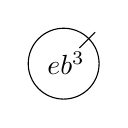
\begin{tikzpicture} \protect\draw (0,0) circle (0.45cm) node {\protect$\leibdashv\, eb^3$}; \protect\draw (.2,.2) -- (.4,.4); \protect\end{tikzpicture}} \;
\leibvdash\, ea^2\cancel{b} \;
\protect\raisebox{-4.5mm}{\protect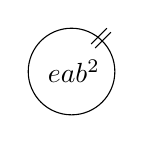
\begin{tikzpicture} \protect\draw (0,0) circle (0.55cm) node at (0,0) {\protect$\leibvdash \,eab^2$}; \protect\draw (.3,.3) -- (.5,.5); \protect\draw (.25,.35) -- (.45,.55); \protect\end{tikzpicture}}\;
\protect\raisebox{-3.5mm}{\protect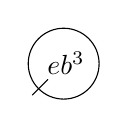
\begin{tikzpicture} \protect\draw (0,0) circle (0.45cm) node {\protect$\leibvdash \,eb^3$}; \protect\draw (-.4,-.4) -- (-.2,-.2); \protect\end{tikzpicture}} \;
\protect\raisebox{-4.5mm}{\protect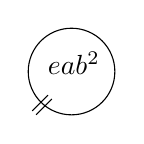
\begin{tikzpicture} \protect\draw (0,0) circle (0.55cm) node at (0,.1) {\protect$\leibdashv \,eab^2$}; \protect\draw (-.3,-.3) -- (-.5,-.5); \protect\draw (-.25,-.35) -- (-.45,-.55); \protect\end{tikzpicture}}\;
\leibvdash\, ea^2\cancel{b}}{ab + b^2} \ $
$\sqcap \ e, \displaystyle\frac{a}{b}, \displaystyle\frac{\leibdashv \;b\; \leibvdash \;2a}{a + b}.$
%
\edtext{}{\lemma{\textit{Am Rand:}}\Afootnote{%
$\leibdashv \sqcap +$}}
%
\pend%
\vspace{1.5em}%
%
\pstart%
\noindent%
\lbrack\textit{Nachfolgend kleingedruckter Text in L gestrichen:}\rbrack\
\pend%
\vspace{0.5em}%
%
\pstart%
\noindent%
{\footnotesize%
% \rule[-3mm]{0pt}{8mm}%
Seu $e, \displaystyle\frac{a}{b},\; \pleibdashv\, 1-\displaystyle\frac{a}{a + b}$ 
aequ. $ e, \displaystyle\frac{a}{b},\; \pleibdashv \displaystyle\frac{b}{a + b}$ aequ.
%calc
$e, \displaystyle\frac{a}{b}, \displaystyle\frac{\protect\raisebox{-1.5mm}{\protect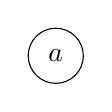
\begin{tikzpicture} \protect\draw (0,0) circle (0.35cm) node {$\leibdashv a$};\protect\end{tikzpicture}}\; \protect\leibdashv b \;
{\protect\raisebox{-1.5mm}{\protect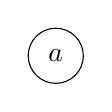
\begin{tikzpicture} \protect\draw (0,0) circle (0.35cm) node {$\leibvdash a$};\protect\end{tikzpicture}}}}{a + b}$\
aequ. $\displaystyle e, \frac{a}{b},\; \pleibdashv\, \displaystyle\frac{b}{a + b},$
aequ. $e,\; \pleibdashv\, \displaystyle\frac{a}{a + b},$
id est \textit{(C)((C))} aequ. \textit{C(C)};
quod est memorabile seu via centri gravitatis manet eadem.%
\rule[-0mm]{0pt}{4mm}%
}%
% $\leibdashv \sqcap +$
% \lbrack\textit{Rechnung bricht ab.}\rbrack\
% \newline}}
\pend%
%\newpage
% \vspace{0.5em}%
\pstart%
\edtext{Ex%
\protect\label{LH_35_09_23_006r_MargDeIIoIIa}%
\edlabel{LH_35_09_23_006r_viacentrigrav_mesj-1}
his
%
\edtext{apparet hic
eandem non}{%
\lemma{apparet}\Bfootnote{%
\textit{(1)}~non
\textit{(2)}~et
\textit{(3)}~hic eandem non%
~\textit{L}}}
%
posse manere viam centri
%
\edtext{gravitatis.
Nihil}{%
\lemma{gravitatis}\Bfootnote{\hspace{-0,5mm}%
\textbar~, nec alia superiorum calculorum\protect\index{Sachverzeichnis}{calculus} compendia\protect\index{Sachverzeichnis}{compendium calculi} hinc observari patet etiam hinc si 2\textit{b} aequ. \textit{a} centrum gravitatis quiescere\protect\index{Sachverzeichnis}{centrum gravitatis quiescens} post concursum. \textit{gestr.}~%
\textbar\ Nihil%
~\textit{L}}}
%
est tamen quod me a sententia%
\protect\index{Sachverzeichnis}{sententia}
demovere possit.
Nam
%
\edtext{si facias}{%
\lemma{si}\Bfootnote{%
\textit{(1)}~faciamus
\textit{(2)}~facias%
~\textit{L}}}
%
$b \sqcap a$ videbis recte omnia procedere.%
\edlabel{LH_35_09_23_006r_viacentrigrav_mesj-2}%
}{\lemma{\textit{Am Rand:}}\Afootnote{%
Non mirari debemus\textsuperscript{[a]}
non manere viam centri gravitatis%
\protect\index{Sachverzeichnis}{via centri gravitatis}%
\protect\index{Sachverzeichnis}{centrum gravitatis}
vel distantiam eandem,%
\protect\index{Sachverzeichnis}{distantia corporum post concursum}
nam utrumque
nisi motu perpetuo admisso%
\protect\index{Sachverzeichnis}{motus perpetuus artificialis}
impossibile esse
demonstravi peculiari scheda%
\textsuperscript{[b]}
secundo secunda hic%
\textsuperscript{[c]}
inserta.%
\protect\index{Sachverzeichnis}{scheda inserta}
% \quad
\lbrack\textit{Nachträglich hinzugefügt:}\rbrack\
Imo paralogismus in illa scheda.%
\protect\index{Sachverzeichnis}{paralogismus}
\newline%
\newline%
{\footnotesize%
\textsuperscript{[a]}~debemus
\textit{(1)}~nec
\textit{(2)}~non%
~\textit{L}
\quad
\textsuperscript{[b]}~scheda secundo secunda:
Vgl. N.~\ref{dcc_02-2}, %??S01\textsubscript{3}, 
S.~\refpassage{LH_35_09_23_004v_motusperpetuus_nnxh-1}{LH_35_09_23_004v_motusperpetuus_nnxh-2}.
\quad
\textsuperscript{[c]}~hic
\textit{erg.~L}%
% \newline%
}}}
\pend%
%
\pstart%
Praeterea,
si parallelogrammum absolvamus%
\protect\index{Sachverzeichnis}{parallelogrammum absolutum}
%
\edtext{fig.~5,}{%
\lemma{fig.~5}\Cfootnote{%
Das Diagramm \lbrack\textit{Fig.~1}\rbrack\ auf S.~\pageref{LH_35_09_23_003,006_Fig.1}.}}
%
patet vim quae communicatur corpori%
\protect\index{Sachverzeichnis}{vis communicata}
in quod incurritur
esse complementum $\delta\lambda,$
eam autem vim continue crescere,
prout corpus incurrens%
\protect\index{Sachverzeichnis}{corpus incurrens}
%
\edtext{crescit\lbrack,\rbrack\
cum contra vis}{%
\lemma{crescit}\Bfootnote{%
\textit{(1)}~vi
\textit{(2)}~cum contra vis%
~\textit{L}}}
%
repulsae $\gamma\delta$ crescat%
\protect\index{Sachverzeichnis}{vis repulsae}
prout corpus repellens crescit,%
\protect\index{Sachverzeichnis}{corpus repellens}
%
\edtext{et eadem est progressio%
\protect\index{Sachverzeichnis}{progressio}
qua vis repulsae crescit%
\protect\index{Sachverzeichnis}{vis repulsae}
incremento excipientis supra aequalitatem,%
\protect\index{Sachverzeichnis}{corpus excipiens}}{%
\lemma{et}\Bfootnote{%
\textit{(1)}~videtur
\textit{(2)}~eadem est
\textit{(a)}~ratio qua vis repellens crescit per impulsam
\textit{(b)}~progressio qua vis repulsae crescit
\textit{(aa)}~proportione repellentis usque ad aequa
\textit{(bb)}~incremento
\textit{(aaa)}~repellentis
\textit{(bbb)}~excipientis supra aequalitatem,%
~\textit{L}}}
%
cum illa
qua vis impulsus crescit%
\protect\index{Sachverzeichnis}{vis impulsus}
(\protect\vphantom)%
incremento seu ascensu impellentis versus aequalitatem,%
\protect\index{Sachverzeichnis}{corpus impellens}
seu%
\protect\vphantom()
decremento excipientis infra
%
\edtext{aequalitatem.
Id est progressio ipsarum $\gamma\delta$
ab \textit{x} versus \textit{z}
est eadem
cum progressione ipsarum $\lambda\delta$ a $\beta$
versus $\theta$,%
\protect\index{Sachverzeichnis}{progressio}
unde sequitur necessario $\beta\delta x$}{%
\lemma{aequalitatem.}\Bfootnote{%
\textit{(1)}~Quo posito $\beta\delta x$
\textit{(2)}~Id est \lbrack...\rbrack\ progressione ipsarum $\lambda\delta$
\textit{(a)}~ab
\textit{(b)}~a $\beta$ \lbrack...\rbrack\ necessario $\beta\delta x$%
~\textit{L}}}
%
esse rectam,%
\protect\index{Sachverzeichnis}{linea recta}
qui modus probandi notandus est.%
\protect\index{Sachverzeichnis}{modus probandi}
Item vis repulsae crescit%
\protect\index{Sachverzeichnis}{vis repulsae}
incremento excipientis supra aequalitatem,
%
\edtext{quemadmodum supra vis impulsus crescebat%
\protect\index{Sachverzeichnis}{vis impulsus}
decremento excipientis infra aequalitatem.}{%
\lemma{quemadmodum \lbrack...\rbrack\ aequalitatem}\Cfootnote{%
Vgl. N.~\ref{dcc_01}, %??S01\textsubscript{1}, 
S.~\refpassage{LH_35_09_23_002r_vobsgos-1}{LH_35_09_23_002r_vobsgos-2}.}}
%
\lbrack6~v\textsuperscript{o}\rbrack\
%
\pend%
\pstart%
Nimirum quatuor habemus propositiones certas%
\protect\index{Sachverzeichnis}{propositio certa}%
\lbrack:\rbrack\
\pend%
\newpage%
%
%
\count\Bfootins=1000%
\count\Afootins=1200%
\count\Cfootins=1000%
\pstart%
\noindent%
%
\edtext{}{%
{\xxref{LH_35_09_23_006v_brsflr-1}{LH_35_09_23_006v_brsflr-2}}%
{\lemma{\textit{Am Rand:}}\Afootnote{%
Hae propositiones manent certae,
etiam postquam aliarum paralogis\-mum deprehendimus.%
\protect\index{Sachverzeichnis}{paralogismus}\vspace{-4mm}%
% \newline
}}}%
\edtext{\textls{I\textsuperscript{o}}%
\edlabel{LH_35_09_23_006v_brsflr-1}%
\textls{ cum incurrens est majus, excipiens minus }%
\edtext{\textls{fig.~7}}{%
\lemma{\textls{fig.~7}}\Cfootnote{Das Diagramm \lbrack\textit{Fig.~3}\rbrack\ auf S.~\pageref{LH_35_09_23_003,006_Fig.3}.}}%
}{%
\lemma{\textls{I\textsuperscript{o}}}\Bfootnote{%
\hspace{-0,5mm}\textls{cum} \lbrack...\rbrack\ \textls{minus fig.~7}
\textit{erg.~L}}}%
\protect\index{Sachverzeichnis}{corpus incurrens majus}%
\protect\index{Sachverzeichnis}{corpus excipiens minus}%
\protect\index{Sachverzeichnis}{figura}
\pend%
%
\pstart%
\noindent%
\hangindent=7,5mm%
%
\edtext{\lbrack1\rbrack}{%
\lemma{\lbrack1\rbrack}\Cfootnote{%
Eckige Klammern von Leibniz.}}
%
Vis progressus%
\protect\index{Sachverzeichnis}{vis progressus}
%
\edtext{$\gamma\delta$}{%
\lemma{$\gamma\delta$}\Bfootnote{
\textit{erg.~L}}}
%
incurrentis \textit{xz}%
\protect\index{Sachverzeichnis}{incrementum incurrentis}
crescit pro incremento ejus
%
\edtext{$x\gamma$}{%
\lemma{$x\gamma$}\Bfootnote{%
\textit{erg.~L}}}
%
supra aequalitatem
%
\edtext{cum $z\gamma$}{%
\lemma{cum}\Bfootnote{%
$z\gamma$
\textit{erg.~L}}}
%
(\protect\vphantom)%
seu pro decremento $x\gamma$ excipientis $z\gamma$ infra aequalitatem cum \textit{zx}.%
\protect\index{Sachverzeichnis}{decrementum excipientis}%
\protect\vphantom()
\pend%
%
\pstart%
\noindent%
\hangindent=7,5mm%
%
\edtext{\lbrack2\rbrack}{%
\lemma{\lbrack2\rbrack}\Cfootnote{%
Eckige Klammern von Leibniz.}}
%
Vis impulsus\protect\index{Sachverzeichnis}{vis impulsus}
%
\edtext{$\lambda\delta$}{%
\lemma{$\lambda\delta$}\Bfootnote{%
\textit{erg.~L}}}
%
recepti in excipiente
%
\edtext{$\beta\lambda$ vel $z\gamma$}{%
\lemma{$\beta\lambda$}\Bfootnote{%
\hspace{-0,5mm}vel $z\gamma$
\textit{erg.~L}}}
%
crescit pro incremento%
\protect\index{Sachverzeichnis}{incrementum excipientis}
%
\edtext{ejus $\beta\lambda$ versus}{%
\lemma{ejus}\Bfootnote{%
\textbar~$\beta\lambda$ \textit{erg.}~\textbar\
\textit{(1)}~supra
\textit{(2)}~versus%
~\textit{L}}}
%
aequalitatem
%
\edtext{cum $\beta\theta$ vel \textit{zx}}{%
\lemma{cum}\Bfootnote{%
\hspace{-0,5mm}$\beta\theta$ vel \textit{zx}
\textit{erg.~L}}}
%
(\protect\vphantom)%
seu pro decremento
%
\edtext{$\beta\lambda$}{%
\lemma{$\beta\lambda$}\Bfootnote{%
\textit{erg.~L}}}
%
\edtext{incurrentis $\beta\theta$
invariati versus aequalitatem%
\protect\index{Sachverzeichnis}{decrementum incurrentis}}{%
\lemma{incurrentis}\Bfootnote{%
\textit{(1)}~\textbar~$\beta\theta$ \textit{erg.}~\textbar\ infra
\textit{(2)}~$\beta\theta$
\textit{(a)}~versus aequalitatem
\textit{(b)}~invariati versus aequalitatem%
~\textit{L}}}
%
cum $\beta\lambda,$
nam incrementum ipsius $\beta\lambda$
in casu ipsius $\beta\theta$ invariati
est decrementum ipsius $\beta\theta$
versus aequalitatem%
\protect\vphantom().
\pend%
% \newpage
% \vspace{0.5em}%
%
\pstart%
\noindent%
\textls{II\textsuperscript{o}
cum incurrens est minus, excipiens majus }%
\edtext{\textls{fig.~8}}{\lemma{\textls{fig.~8}}\Cfootnote{Das Diagramm \lbrack\textit{Fig.~4}\rbrack\ auf S.~\pageref{LH_35_09_23_003,006_Fig.4}.}}%
\protect\index{Sachverzeichnis}{corpus incurrens minus}%
\protect\index{Sachverzeichnis}{corpus excipiens majus}
\pend%
%
\pstart%
\noindent%
\hangindent=7,5mm%
%
\edtext{\lbrack3\rbrack}{%
\lemma{\lbrack3\rbrack}\Cfootnote{%
Eckige Klammern von Leibniz.}}
%
Vis repulsae%
\protect\index{Sachverzeichnis}{vis repulsae}
%
\edtext{$\gamma\delta$}{%
\lemma{$\gamma\delta$}\Bfootnote{%
\textit{erg.~L}}}
%
incurrentis
%
\edtext{$z\gamma$}{%
\lemma{$z\gamma$}\Bfootnote{%
\textit{erg.~L}}}
%
crescit pro
%
\edtext{decremento ejus $x\gamma$%
\protect\index{Sachverzeichnis}{decrementum incurrentis}}{%
\lemma{decremento}\Bfootnote{%
\textit{(1)}~\textbar~$x\gamma$ \textit{streicht Hrsg.}~\textbar\
\textit{(2)}~ejus $x\gamma$%
~\textit{L}}}
%
infra aequalitatem
%
\edtext{cum \textit{zx},}{%
\lemma{cum}\Bfootnote{%
\hspace{-0,5mm}\textit{zx}
\textit{erg.~L}}}
%
seu pro incremento
%
\edtext{$x\gamma$}{%
\lemma{$x\gamma$}\Bfootnote{%
\textit{erg.~L}}}
%
excipientis%
\protect\index{Sachverzeichnis}{decrementum excipientis}
%
\edtext{\textit{zx}}{%
\lemma{\textit{zx}}\Bfootnote{
\textit{erg.~L}}}
%
supra aequalitatem cum $z\gamma$.
\pend
%
\pstart%
\noindent%
\hangindent=7,5mm%
%
\edtext{\lbrack4\rbrack}{%
\lemma{\lbrack4\rbrack}\Cfootnote{%
Eckige Klammern von Leibniz.}}
%
Vis impulsus $\lambda\delta$%
\protect\index{Sachverzeichnis}{vis impulsus}
recepti in excipiente $\beta\theta$
crescit pro decremento ejus%
\protect\index{Sachverzeichnis}{decrementum excipientis}
%
\edtext{$\beta\lambda$ versus}{%
\lemma{$\beta\lambda$}\Bfootnote{%
\textit{(1)}~infra
\textit{(2)}~versus%
~\textit{L}}}
%
aequalitatem,
id est,
quia ipsum ut invariatum consideratur%
\lbrack,\rbrack\
pro
%
\edtext{incremento ipsius excipientis $\beta\lambda$%
\protect\index{Sachverzeichnis}{incrementum excipientis}}{%
\lemma{incremento}\Bfootnote{%
\textit{(1)}~\textbar~$\beta\lambda$ \textit{streicht Hrsg.}~\textbar\
\textit{(2)}~ipsius excipientis $\beta\lambda$%
~\textit{L}}}
%
versus aequalitatem
%
\edlabel{LH_35_09_23_003,006_concursu15}% % ex-label: concursu15
cum $\beta\theta.$%
\edlabel{LH_35_09_23_006v_brsflr-2}%
\edtext{}{%
{\xxref{LH_35_09_23_003,006_concursu15}{LH_35_09_23_003,006_concursu16}}%
\lemma{cum}\Bfootnote{%
\textit{(1)}~ipso
\textit{(2)}~$\beta\theta$
\textit{(a)}~Poterimus et alias enuntiare propositiones sumendo
\textit{(b)}~Hae propositiones%
~\textit{L}}}%
%
\pend%
%
\pstart%
\noindent%
Hae propositiones%
\edlabel{LH_35_09_23_003,006_concursu16} % ex-label: concursu16
ex prioribus certae sunt,%
\protect\index{Sachverzeichnis}{propositio certa}
sed non sequitur hinc lineam $\beta\delta x$ esse rectam,%
\protect\index{Sachverzeichnis}{linea recta}
seu quando dicitur aliquid crescere
pro alterius incremento vel decremento,
crescere in eadem cum eo ratione;
%
\edtext{nisi ponendo eandem esse}{%
\lemma{nisi}\Bfootnote{%
\textit{(1)}~constet
\textit{(2)}~ponendo eandem esse%
~\textit{L}}}
%
progressionem\protect\index{Sachverzeichnis}{progressio}
in prop.~2 quae in prop.~1,
et in prop.~4 quae in prop.~3.
\pend%
%\newpage%
%
\pstart%
Unaquaeque ex his propositionibus est
%
\edtext{duplicata.
Seu virtute}{%
\lemma{duplicata.}\Bfootnote{%
\textit{(1)}~Et si vis
\textit{(2)}~Seu virtute%
~\textit{L}}}
%
sunt octo,
et si pro virium incremento substitueretur decrementum,%
\protect\index{Sachverzeichnis}{incrementum virium}%
\protect\index{Sachverzeichnis}{decrementum virium}
fierent aliae octo,
in summa 16.
\pend%
\pstart%
Aliae figurae condi possunt%
\protect\index{Sachverzeichnis}{figura}
in quibus invariato manente minore,
mutatur majus.
\pend%
\newpage
\pstart 
%\noindent
\begin{minipage}[t]{0.5\textwidth}
\includegraphics[width=0.72\textwidth]{gesamttex/edit_VIII,3/images/LH_35_09_23_003,006_d3.pdf}
\end{minipage}
\hspace{0mm}
\begin{minipage}[t]{0.5\textwidth}
\includegraphics[width=0.83\textwidth]{gesamttex/edit_VIII,3/images/LH_35_09_23_003,006_d4.pdf}
\end{minipage}
\\
\\
\hspace*{25mm} [\textit{Fig.~3}]\hspace*{60mm} [\textit{Fig.~4}]\label{LH_35_09_23_003,006_Fig.3}\label{LH_35_09_23_003,006_Fig.4}%
\pend
\vspace{1.5em}
%%
%%  \newpage% 
%  \centerline{\hspace{-80mm}\includegraphics[width=0.36\textwidth]{gesamttex/edit_VIII,3/images/LH_35_09_23_003,006_d3.pdf}}%
%  \vspace*{0.5em}
%  \centerline{\hspace{-80mm}\lbrack\textit{Fig.~3}\rbrack}%
%  \label{LH_35_09_23_003,006_Fig.3}%
%%  \vspace{1.5em}%
%  \vspace*{-14.5em}%	% Diagramm 4
%  \centerline{\hspace{80mm}\includegraphics[width=0.42\textwidth]{gesamttex/edit_VIII,3/images/LH_35_09_23_003,006_d4.pdf}}%
%  \vspace*{0.25em}
%  \centerline{\hspace{80mm}\lbrack\textit{Fig.~4}\rbrack}%
%  \label{LH_35_09_23_003,006_Fig.4}%
%  \vspace{1.25em}%
%%  \newpage%
%%
%%
\pstart%
Jungamus\setline{1}\edtext{%
\edlabel{LH_35_09_23_006v_skbc-1}
inter se majus et minus}{%
\lemma{Jungamus}\Bfootnote{%
\hspace{-0,5mm}inter % se majus 
\lbrack...\rbrack\ et minus
\textit{erg.~L}}}%
\lbrack:\rbrack\
%
\edtext{I\textsuperscript{o}
cum incurrens\protect\index{Sachverzeichnis}{corpus incurrens varians}
%
\edtext{variatur excipiens%
\protect\index{Sachverzeichnis}{corpus excipiens invarians}}{%
\lemma{variatur}\Bfootnote{%
\textit{(1)}~majus
\textit{(2)}~excipiens%
~\textit{L}}}
%
manet,}{\lemma{I\textsuperscript{o} cum \lbrack...\rbrack\ manet}\Cfootnote{%
Der symmetrische zweite Fall,
bei dem der stoßende Körper unverändert bleibt und der gestoßene variiert,
wird erst in der \textit{Scheda III} (N.~\ref{dcc_03}, %??S01\textsubscript{4}, 
S.~\refpassage{LH_35_09_23_007r_xddg-1}{LH_35_09_23_007r_xddg-2}) besprochen.
Vgl. auch die Variante \textit{(2)} zum Textabschnitt $\textit{(}\gamma\textit{)(}\lambda\textit{)}.$ \textit{Notanda permutatio est}, S.~\refpassage{LH_35_09_23_003,006_concursu17}{LH_35_09_23_003,006_concursu18}.}}
%
fig.~8.
%\edtext{%
Vis vel repulsae%
\protect\index{Sachverzeichnis}{vis repulsae}
vel progressus,%
\protect\index{Sachverzeichnis}{vis progressus}
%}{%
%\lemma{Vis \lbrack...\rbrack\ progressus}\Cfootnote{%
%Wie auch an anderen Stellen im Haupttext der Fall ist, verwendet Leibniz hier \textit{vis} und \textit{celeritas} als gleichbedeutend.
%Die Gleichsetzung ist jedoch nicht in jedem Kontext berechtigt.}}
%
id est vis
%
\edtext{retenta incurrentis
$\beta\lambda$ est in fig. 8%
\protect\index{Sachverzeichnis}{figura}
ordinata $\delta\gamma$}{%
\lemma{retenta}\Bfootnote{\hspace{-0,5mm}%
\textit{(1)}~$\lambda\delta$
\textit{(2)}~incurrentis $\beta\lambda$
\textit{(a)}~crescit pro magnitudine ipsius incurrentis, id est si magni%
\protect\index{Sachverzeichnis}{magnitudo corporis incurrentis}
\textit{(b)}~\textlangle\textendash\ sit\textrangle\
\textit{(c)}~est in fig. 8 ordinata $\delta\gamma$%
~\textit{L}}}
%
a linea $\beta\delta x\textit{(}\delta\textit{)}$
ad rectam $z\gamma x\textit{(}\gamma\textit{)},$
sive $\gamma\delta$ vel $\textit{(}\gamma\textit{)(}\delta\textit{)}$
celeritas incurrentis $z\gamma$ vel $z\textit{(}\gamma\textit{)}$
post concursum est%
\protect\index{Sachverzeichnis}{celeritas post concursum}
%
\edtext{ad vim}{%
\lemma{ad}\Bfootnote{%
\textit{(1)}~celeritatem
\textit{(2)}~vim%
~\textit{L}}}
%
\edlabel{LH_35_09_23_006v_fhgscfdbh-1}%
\edtext{incursus%
\protect\index{Sachverzeichnis}{vis incursus}
seu rectam
%
\edtext{\lbrack$\delta\lambda$\rbrack\ vel \lbrack$\textit{(}\delta\textit{)(}\lambda\textit{)}$\rbrack}{%
\lemma{\lbrack$\delta\lambda$\rbrack\ vel \lbrack$\textit{(}\delta\textit{)(}\lambda\textit{)}$\rbrack}\Cfootnote{%
Dem Text liegt offenbar eine Schwankung zwischen der konstanten \textit{celeritas incursus} $z\beta$ (bzw. $\gamma\lambda$ bzw. $x\theta$) und der variablen, von der Masse des stoßenden Körpers abhängigen \textit{vis incursus} zugrunde.
Die besagte Schwankung wird besonders in der Variante\,\textit{(2a)} zum Textabschnitt \textit{incursus} \lbrack...\rbrack\ $z\gamma$ \textit{vel} $z\textit{(}\gamma\textit{)}$ (S.~\refpassage{LH_35_09_23_006v_fhgscfdbh-1}{LH_35_09_23_006v_fhgscfdbh-2}) deutlich.
Siehe auch \textsc{Fichant} 1994,\cite{01056} S.~87, Anm.~3.}}
%
ut differentia magnitudinum%
\protect\index{Sachverzeichnis}{differentia magnitudinum}
$x\gamma$ vel $x\textit{(}\gamma\textit{)}$ ad
\edtext{corpus \lbrack minus\rbrack\ $z\gamma$ vel $z\textit{(}\gamma\textit{)}.$}{%
\lemma{corpus \lbrack minus\rbrack\ $z\gamma$ vel $z\textit{(}\gamma\textit{)}$}\Cfootnote{%
Siehe hierüber \cite{01056}\textsc{Fichant} 1994, S.~87, Anm.~4.}}%
}{%
\lemma{incursus}\Bfootnote{%
\textit{(1)}~$x\theta$ vel $\textit{(}x\textit{)(}\theta\textit{)}$
\textit{(2)}~seu rectam
\textbar~$\gamma\lambda$ \textit{ändert Hrsg.}~%
\textbar\ vel 
\textbar~$\textit{(}\delta\textit{)}\lambda$ \textit{ändert Hrsg.}~%
\textbar\
\textit{(a)}~(\protect\vphantom)sed haec expressio non placet, quia hoc modo variatur vis incursus, quam eandem manere volebam, non minus ac excipiens,
\textit{(b)}~\textbar~id est \textit{streicht Hrsg.}~\textbar\
\textit{(c)}~ut differentia \lbrack...\rbrack\ ad corpus
\textbar~majus \textit{ändert Hrsg.}~%
\textbar\ $z\gamma$ vel $z\textit{(}\gamma\textit{)}.$%
~\textit{L}}}%
\edlabel{LH_35_09_23_006v_fhgscfdbh-2}
%
\edtext{}{%
{\xxref{LH_35_09_23_006v_oibk-1}{LH_35_09_23_006v_oibk-2}}%
{\lemma{\textit{Am Rand:}}\Afootnote{%
Haec vera manent.
% \newline%
}}}%
%
\edlabel{LH_35_09_23_006v_oibk-1}%
Hinc sequetur illud
%
%
\edtext{memorabile,
incurrente}{%
\lemma{memorabile,}\Bfootnote{%
\textit{(1)}~excipiente
\textit{(2)}~incurrente%
~\textit{L}}}
%
$z\textit{(}\gamma\textit{)}$ utcunque
%
\edtext{crescente super excipiens,}{%
\lemma{crescente}\Bfootnote{%
\textit{(1)}~et
\textit{(2)}~vim communicatam\protect\index{Sachverzeichnis}{vis communicata}
\textit{(3)}~super excipiens%
~\textit{L}}}
%
et vi%
\protect\index{Sachverzeichnis}{vis corporis incurrentis}
%
\edtext{seu
\edtext{(h.\,l.)}{\lemma{(h.\,l.)}\Cfootnote{\textit{hoc loco}}}
celeritate%
\protect\index{Sachverzeichnis}{celeritas corporis incurrentis}%
}{%
{\lemma{seu}\Bfootnote{%
\hspace{-0,5mm}(h.\,l.) celeritate
\textit{erg.~L}}}%
{\lemma{seu (h.\,l.) celeritate}\Cfootnote{%
Die Gleichsetzung von \textit{vis} und \textit{celeritas} ist gerade an dieser Stelle nicht zulässig. Denn die Stoßgeschwindigkeit $z\beta$ bzw. $\gamma\lambda$ bleibt hier konstant, während die Stoßkraft je nach Variierung der Masse des stoßenden Körpers variiert.}}%
}
%
incurrentis\protect\index{Sachverzeichnis}{corpus incurrens}
%
\edtext{\lbrack$\textit{(}\delta\textit{)(}\lambda\textit{)}$\rbrack}{%
\lemma{$\delta\lambda$}\Bfootnote{%
\textit{erg.~L, ändert Hrsg.}}}
%
proportionaliter
%
\edtext{crescente,
vim impulsus%
\protect\index{Sachverzeichnis}{vis impulsus}}{%
\lemma{crescente,}\Bfootnote{%
\textit{(1)}~impulsum
\textit{(2)}~vim impulsus%
~\textit{L}}}
%
ab excipiente suscepti
manere eandem
\edlabel{LH_35_09_23_003,006_concursu17}% % ex-label: concursu17
$\textit{(}\gamma\textit{)(}\lambda\textit{)}.$%
\edlabel{LH_35_09_23_006v_oibk-2}%
%
%
\edtext{}{%
{\xxref{LH_35_09_23_003,006_concursu17}{LH_35_09_23_003,006_concursu18}}%
{\lemma{$\textit{(}\gamma\textit{)(}\lambda\textit{)}$.}\Bfootnote{%
\textit{(1)}~Contra incurrente $z\textit{(}\gamma\textit{)}$ utcunque decrescente et vi incursus\protect\index{Sachverzeichnis}{vis incursus} eadem manente $\gamma\lambda$
\textit{(2)}~II\textsuperscript{o} cum
\textit{(3)}~Nota
\textit{(4)}~Notanda permutatio est%
~\textit{L}}}}%
\pend%
% \newpage%
%
\pstart%
Notanda permutatio est%
\protect\index{Sachverzeichnis}{permutatio}%
\edlabel{LH_35_09_23_003,006_concursu18} % ex-label: concursu18
in figura~8,%
\protect\index{Sachverzeichnis}{figura}
nempe
manente excipiente,
et observatis regulis nostris,%
\protect\index{Sachverzeichnis}{regulae concursus}
$\delta\lambda$
quae erat primum excipientis%
\protect\index{Sachverzeichnis}{corpus excipiens}
%
\edtext{\textit{zx},
\lbrack fit\rbrack\
postea $\textit{(}\delta\textit{)(}\lambda\textit{)}$ incurrentis%
\protect\index{Sachverzeichnis}{corpus incurrens}}{%
\lemma{\textit{zx},}\Bfootnote{%
\textit{(1)}~fit
\textit{(2)}~\textbar~et \textit{ändert Hrsg.}~%
\textbar\ postea $\textit{(}\delta\textit{)(}\lambda\textit{)}$
\textbar~fit \textit{streicht Hrsg.}~%
\textbar\ incurrentis%
~\textit{L}}}
%
\edtext{$\textit{z(}\gamma\textit{)},$
item $\gamma\lambda$ erat primum incursus,%
\protect\index{Sachverzeichnis}{incursus}
fit postea
$\textit{(}\gamma\textit{)(}\lambda\textit{)}$
excipientis.
\newline%
\indent%
In eadem fig.~8}{%
\lemma{$z\textit{(}\gamma\textit{)},$}\Bfootnote{%
\textit{(1)}~ea vocetur $\textit{(}\delta\textit{)(}\lambda\textit{)}$
\textit{(2)}~item $\gamma\lambda$
\textit{(a)}~quae erat primum
\textit{(aa)}~excipientis
\textit{(bb)}~incurrentis
\textit{(b)}~erat primum % incursus, fit postea 
\lbrack...\rbrack\ $\textit{(}\gamma\textit{)(}\lambda\textit{)}$ excipientis.
\textit{(aaa)}~Sed jam video figuram nostram nullo modo procedere. \textit{gestr.}~%
\textit{(aa)}~In eadem fig.~8%
~\textit{L}}}
%
vis ab excipiente%
\protect\index{Sachverzeichnis}{vis suscepta}%
\protect\index{Sachverzeichnis}{figura}
%
\edtext{\textit{zx}}{%
\lemma{\textit{zx}}\Bfootnote{%
\textit{erg.~L}}}
%
\edtext{suscepta $\delta\lambda$
crescit continue
in proportione incurrentis\lbrack,\rbrack\
posito
\lbrack celeritatem\rbrack\
incursus%
\protect\index{Sachverzeichnis}{vis incursus}
manere eandem $\gamma\lambda$,
donec}{%
\lemma{suscepta}\Bfootnote{%
\textit{(1)}~manet
\textit{(2)}~$\delta\lambda$ crescit continue in proportione
\textit{(a)}~excipientis
\textit{(b)}~incurrentis
\textbar~posito
\textbar~vim \textit{ändert Hrsg.}~%
\textbar\ incursus manere eandem $\gamma\lambda$ \textit{erg.}~\textbar\ 
\textit{(aa)}~et p
\textit{(bb)}~donec%
~\textit{L}}}
%
excipiens
%
\edtext{\textit{zx}}{%
\lemma{\textit{zx}}\Bfootnote{%
\textit{erg.~L}}}
%
fiat minus incurrente $z\gamma$.
%\pend%
%%
%\pstart%
Nam tunc vi incursus%
\protect\index{Sachverzeichnis}{vis incursus}
$\textit{(}\delta\textit{)(}\lambda\textit{)}$
crescente continue,
vis ab excipiente suscepta manet eadem,
ea scilicet ipsa
quae
%
\edtext{antea}{%
\lemma{antea}\Cfootnote{%
Nämlich zu dem Punkt, als $\displaystyle z\gamma$ und \textit{zx} gleich waren.}}
%
erat vis incursus.
Ut proinde intra vim incursus,%
\protect\index{Sachverzeichnis}{vis incursus}
et vim ab excipiente susceptam%
\protect\index{Sachverzeichnis}{corpus excipiens}%
\protect\index{Sachverzeichnis}{vis suscepta}
elegans sit reciprocatio.%
\protect\index{Sachverzeichnis}{reciprocatio}
\pend%
%
\pstart%
Illud
%
\edtext{nonnihil confusum}{%
\lemma{nonnihil}\Bfootnote{%
\textit{(1)}~animum d
\textit{(2)}~confusum%
~\textit{L}}}
%
videtur,
quod si
%
\edtext{pro vi retenta%
\protect\index{Sachverzeichnis}{vis retenta}
incurrentis%
\protect\index{Sachverzeichnis}{corpus incurrens}
eaedem manent}{%
\lemma{pro}\Bfootnote{%
\textit{(1)}~vi incurrentis eaedem ma
\textit{(2)}~vi retenta incurrentis eaedem manent%
~\textit{L}}}
%
literae in fig.~8,
sive majus sit sive minus excipiente,
non possint tamen eaedem manere literae%
\protect\index{Sachverzeichnis}{litera}
pro vi excipientis et incursus.%
\protect\index{Sachverzeichnis}{vis incursus}%
\protect\index{Sachverzeichnis}{vis corporis excipientis}
Sed qui figuram considerabit,%
\protect\index{Sachverzeichnis}{figura}
facile videbit
quomodocunque linea $\beta\delta x\textit{(}\delta\textit{)}$ conciperetur,
id est etiamsi non esset recta,%
\protect\index{Sachverzeichnis}{linea recta}
tamen id futurum esse.%
\edlabel{LH_35_09_23_006v_skbc-2}
\pend%
%\newpage%
%
\pstart%
\edtext{%
Notandum praeterea posito
%
\edtext{ex praecedentibus}{%
\lemma{ex praecedentibus}\Cfootnote{%
Vgl. N.~\ref{dcc_01}, %??S01\textsubscript{1},
S.~\refpassage{LH_35_09_23_002r_probaturrecta_mxyz-1}{LH_35_09_23_002r_probaturrecta_mxyz-2};
N.~\ref{dcc_02-1}, %??S01\textsubscript{2},
S.~\refpassage{LH_35_09_23_003v_krjhgk-1}{LH_35_09_23_003v_krjhgk-2}.}}
%
$x\textit{(}\delta\textit{)}$ esse rectam,
ubi de incursu majoris in minus agebatur,%
\protect\index{Sachverzeichnis}{corpus majus in minus}
ideo nunc nihil esse credibilius,
quam etiam $x\delta$ esse rectam,
quando de incursu minoris in majus agitur.%
\protect\index{Sachverzeichnis}{corpus minus in majus}%
\protect\index{Sachverzeichnis}{incursus}%
}{%
\lemma{\textit{Am Rand:}}\Afootnote{%
Error utrobique.%
\protect\index{Sachverzeichnis}{error}}}
%
\pend
%
%
% % % %    Ende des Textes auf Bl.~6v